\documentclass[slovak,a4paper]{coursepaper}
\usepackage[12pt]{extsizes}
\usepackage[slovak]{babel}
\usepackage[IL2]{fontenc}
\usepackage[utf8]{inputenc}
\usepackage{hyperref}
\usepackage{float}
\usepackage{pdfpages}
\usepackage{tabularx}
\usepackage{graphicx}

\pagestyle{headings} 
\title{Odporúčacie algoritmy LinkedIn\centering}


\author{Maksym Boiko\\[2pt]
{ Slovenská technická univerzita v Bratislave}\\
{ Fakulta informatiky a informačných technológií}\\
{\texttt{xboikom1@stuba.sk}}\\
{\texttt{Zdroj, ktorý usmernil:~\cite{1}}}
}

\date{\small 07. December 2024}

\begin{document}

\maketitle

\section{Na čo sú určené?}
Odporúčacie algoritmy LinkedIn sú veľmi dôležité pri určovaní informácií, ktoré používatelia vidia vo svojich kanáloch. Ich hlavným cieľom je vytvoriť zaujímavý a hodnotný používateľský zážitok poskytovaním personalizovaného obsahu, ktorý zodpovedá záujmom, preferenciám a profesionálnym potrebám každého používateľa.

V tomto článku budete môcť pochopiť, ako fungujú odporúčacie algoritmy na platforme LinkedIn, a ako tieto znalosti efektívne využiť na propagáciu svojho profilu, spoločnosti alebo rychlo si najst povolanie.~\cite{2}

\section{Actívny rozvoj spoločnosti} \label{rozvoj spoločnosti}

Pre mnohých ľudí LinkedIn je zaroveň aj príležitosťou na profesionálny rozvoj, hľadanie práce a prácovné vzťahy.
Spoločnosť aktívne rozvíja svoje technológie s cieľom zlepšiť používateľskú skúsenosť a poskytovať relevantnejší obsah. V roku 2024 algoritmy LinkedIn sa výrazne zmenili a zameriavajú sa skôr na presnosť obsahu ako na viralitu. To znamená, že používatelia teraz môžu viac zamerať na zdieľanie odborných vedomostí a skúseností, namiesto toho, aby sa snažili o masový dosah. Však, pozrime sa ďalej na kľúčové výhody odporúčacích algoritmov.

\section{Užitočnosť} \label{Užitočnosť}
Algoritmy regulujú mnohé aspekty odporúčaní s cieľom zlepšiť používateľskú skúsenosť a produktivitu. Hlavné z nich sú:

\begin{itemize}
	\item Odporúčania nových kontaktov, ktoré používateľ môže poznať
	\item Pomoc pri hľadaní zamestnania
	\item Výber obsahu pre informačný kanál
	\item Odporúčania týkajúce sa kurzov odbornej prípravy a zručností
	\item Analýza a prognóza kariérneho vývoja
  \end{itemize}

Okrem toho, pochopenie fungovania algoritmov LinkedIn vám umožní efektívnejšie propagovať vašu značku alebo spoločnosť sústredením sa na vytváranie hodnotného obsahu pre správne publikum.~\cite{3}

\newpage
\section{Typy odporúčacích algoritmov} \label{Typy}
V sieti LinkedIn sa používa niekoľko typov odporúčacích algoritmov:


\begin{table}[h!]
    \begin{tabularx}{\textwidth}{|>{\centering\arraybackslash}l|X|}
        \hline
        \textbf{Typ} & \textbf{Ako funguje} 
		\\ \hline Kolaboratívne filtrovanie & Odporúča obsah na základe správania používateľov 
		s podobnými záujmami a interakciami. Napríklad, ak sa niektorý článok páči viacerým ľuďom vo vašej sieti, môže vám byť navrhnutý.

		\\ \hline Filtrovanie obsahu & Odporúča na základe analýzy tém, hashtagov a zručností uvedených v profiloch s cieľom navrhnúť relevantný obsah.  
		\\ \hline Hybridné metódy & LinkedIn kombinuje kolaboratívne filtrovanie a filtrovanie obsahu pre personalizovanejšie odporúčania, napríklad pracovných miest a ľudí.
		\\ \hline Grafové algoritmy & Slúžia na odporúčanie kontaktov vyhľadávaním spojení prostredníctvom spoločných známych alebo spoločných záujmov.
		\\ \hline
    \end{tabularx}
    \label{tab:typy}
\end{table}

Tieto algoritmy pomáhajú zlepšiť interakcie, nájsť užitočné zdroje a rozšíriť vašu sieť.~\cite{4} Na obrázku nižšie môžeme vidieť, ako často sa používajú rôzne typy odporúčacích algoritmov LinkedIn.

\begin{figure}[H]
	\hspace*{-3cm}
	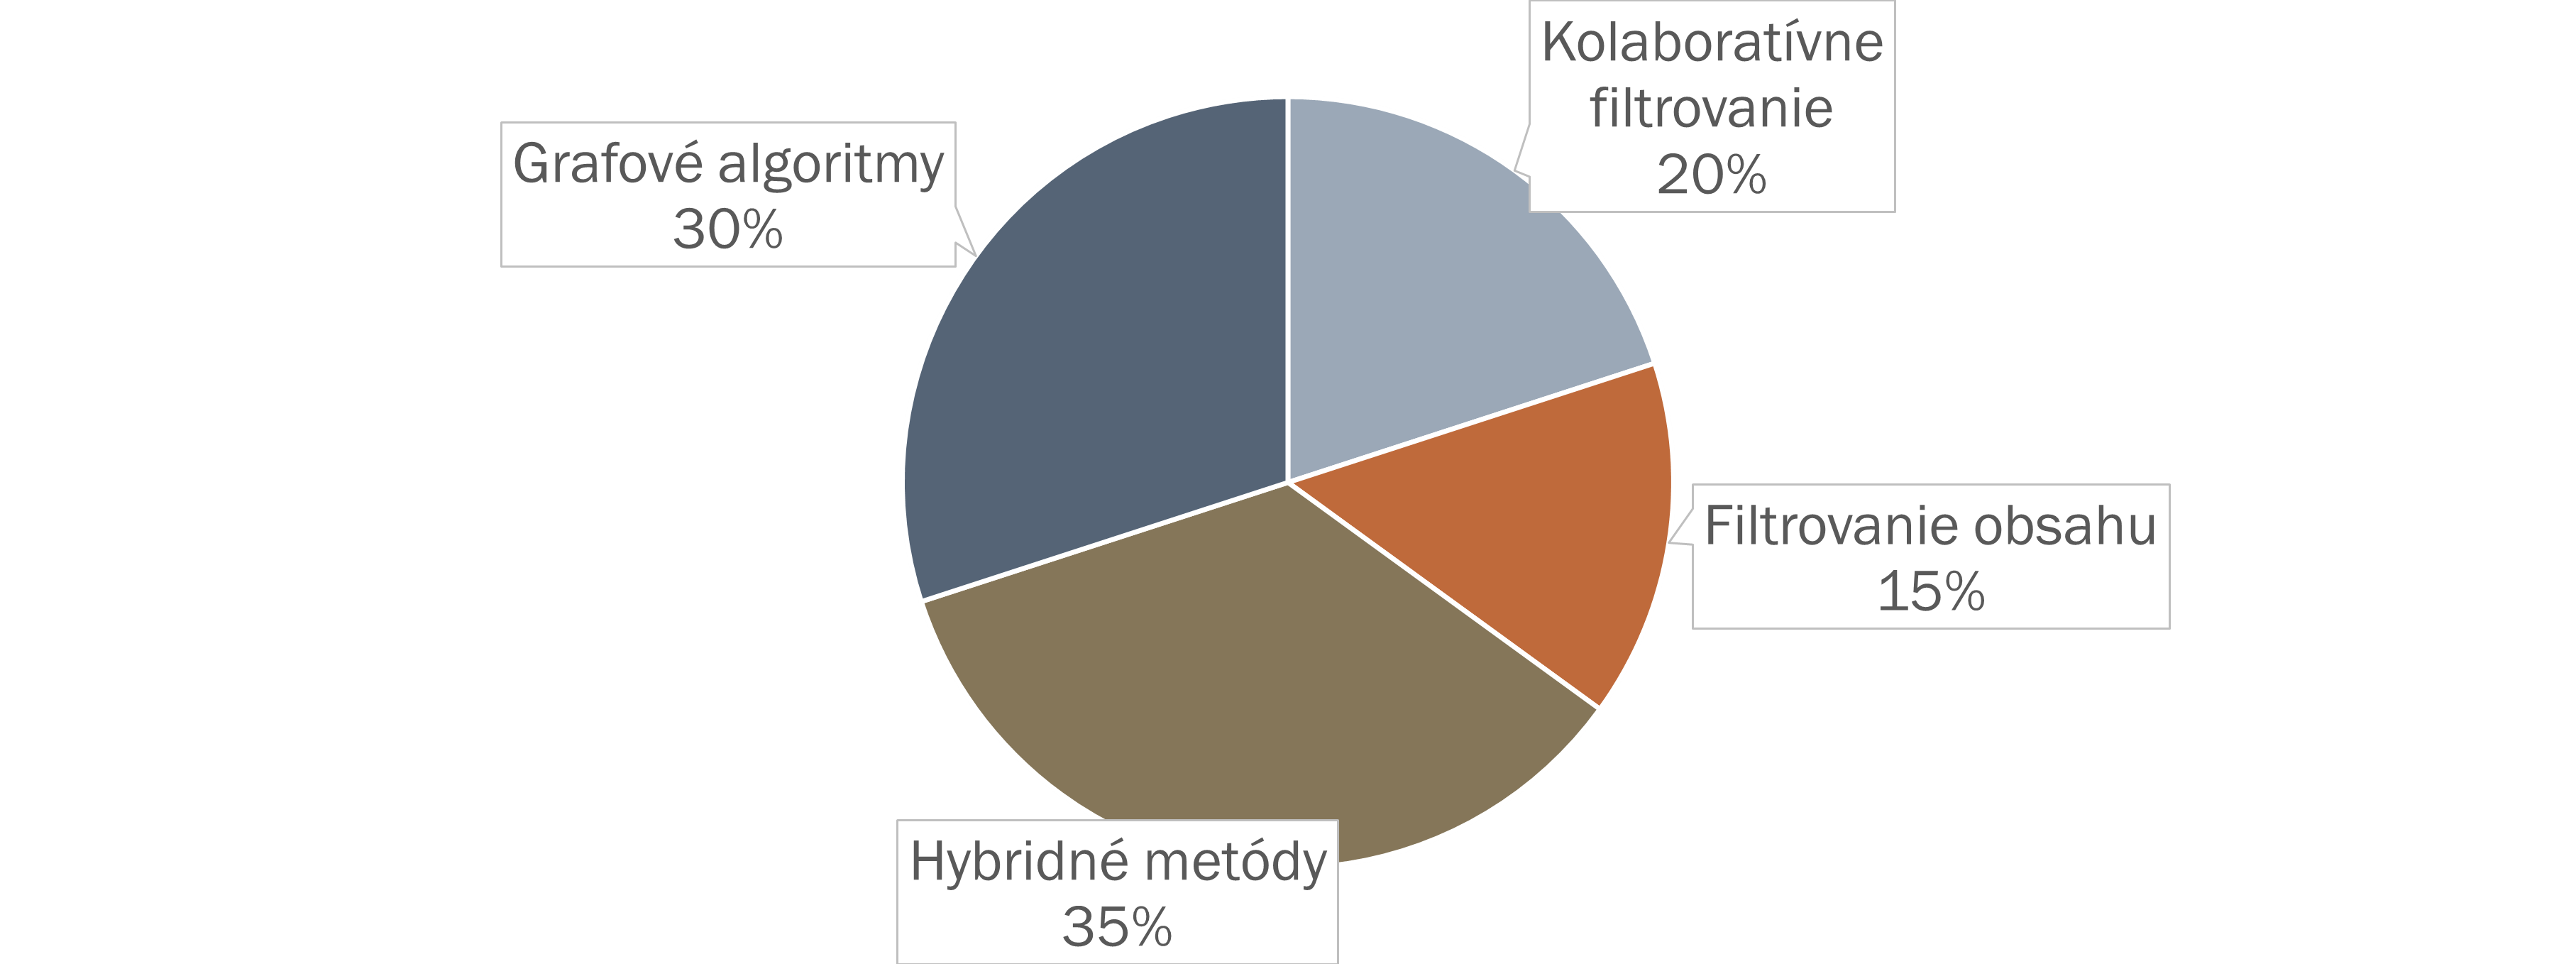
\includegraphics[width=1.4\textwidth]{graph.png}
\end{figure}

Hybridné metódy sa používajú najčastejšie, pretože majú lepšiu personalizáciu. Takéto systémy môžu zohľadňovať explicitné preferencie používateľa a implicitné signály (napr. údaje o prehliadaní a interakcii). Tento prístup umožňuje sieti LinkedIn poskytovať vysoko personalizované odporúčania, napríklad navrhovať pracovné ponuky prispôsobené profilu používateľa a jeho historickému správaniu.~\cite{5}

\section{Ako algoritmy fungujú} \label{fungovanie}
\textbf{Filtrovanie obsahu}: Pozrime sa na odporúčania na príklade publikačných materiálov. Algoritmus LinkedIn používa rôzne faktory na určenie relevantnosti vášho príspevku pre vaše cieľové publikum. Najprv keď niečo zverejníte bot zaradí váš obsah do kategórie spam, nízka kvalita alebo vysoká kvalita podľa hodnoty.~\cite{6}

\textbf{Relevantný obsah}: Platforma sa snaží vyzdvihnúť viac vedomostí a skúseností, o ktoré sa odborníci delia. Pre používateľov algoritmus určuje, ktoré odborné znalosti sú podstatné, pomocou identifikacii záujmov používateľa na základe informácií o jeho profile a činnosti.~\cite{7}

\textbf{Pracovné odporúčania}: LinkedIn umožňuje náborovým pracovníkom vyhľadávať kandidátov na základe ich zručností a skúseností. Navyše poskytuje skvelú platformu na nábor talentovaných zamestnancov, najmä pre začínajúce podniky, ktoré nie sú dostatočne viditeľné v porovnaní s nadnárodnými korporáciami.~\cite{8}

Existuje však aj iný, modernejší typ práce algoritmov - s využitím strojového učenia. Tento prístup umožňuje algoritmom prispôsobovať sa, učiť sa z údajov a zlepšovať svoju presnosť. To dramaticky mení efektivitu a schopnosti systémov LinkedIn a vedie k revolúcii v ich fungovaní.

\section{Vplyv strojového učenia na algoritmy spoločnosti Linkedin} \label{strojové učenie}
Pomocou strojového učenia systém kombinuje niekoľko kľúčových komponentov:
\begin{itemize}
	\item Relevantnosť: algoritmy vyberajú kandidátov, ktorí najlepšie zodpovedajú požiadavkám na pracovné miesto.
	\item Analýza dopytu: rozširuje vyhľadávanie o súvisiace zručnosti a pozície.
	\item Personalizácia: prispôsobuje sa individuálnym preferenciám náborového pracovníka a zlepšuje odporúčania.
\end{itemize}

LinkedIn môže aj využívať umelú inteligenciu na odporúčanie vhodných pracovných príležitostí, poskytovanie návrhov kurzov na zvyšovanie kvalifikácie, navrhovanie náborovým pracovníkom najlepších talentov na voľné pracovné miesta atď.~\cite{9}

\section{Uplatňovanie odporúčaní na rôzne časti platformy} \label{Uplatňovanie}
LinkedIn používa odporúčacie algoritmy na zlepšenie efektívnosti interakcie používateľov s platformou.
Algoritmy môžu pomáhať v rôznych aspektoch fungovania sociálnej siete.
Okrem vyššie uvedených pracovných pokynov a personalizovaného informačného kanála, taktiež sa odporúčajú aj vzdelávací obsah, skupiny a komunity na základe záujmov používateľov, optimalizujú sa reklamné odporúčania.

V roku 2024 sa algoritmus LinkedIn vyvinul tak, aby uprednostňoval obsah, ktorý je pre používateľov najrelevantnejší a najzaujímavejší.
Využíva strategický prístup k marketingu na sieti prostredníctvom analýzy odbornej relevantnosti obsahu na sociálnych platformách, ako je LinkedIn.~\cite{10}


\section{Zbieranie a analýza údajov na účely odporúčaní} \label{analýza údajov}
LinkedIn zbiera a analyzuje veľké množstvo údajov na poskytovanie odporúčaní. Tieto odporúčania sú spracované algoritmami strojového učenia na vytvorenie personalizovaných odporúčaní, ako napríklad pracovných miest, obsahu, ľudí, ktorých si môžete pridať, a kurzov.

Algoritmus sa používa aj na predpovedanie kariéry používateľa a pomáha mu plánovať jeho profesionálny rozvoj. LinkedIn analyzuje interakcie používateľov (lajky, komentáre, reposty), profilové údaje (zručnosti, pracovné skúsenosti, vzdelanie a záujmy) a súvislosti interakcií.~\cite{11}

Analýza platformy pomáha používateľom nájsť správne kariérne príležitosti, rozšíriť sieť kontaktov a zlepšiť svoje publikácie, aby sa dostali k správnemu publiku. Analytické nástroje sú užitočné aj na sledovanie úspešnosti obsahu a pochopenie preferencií cieľového prostredia.

\section{\texorpdfstring{Tipy na zlepšenie účinnosti vášho obsahu na \\ LinkedIn}{Tipy na zlepšenie účinnosti vášho obsahu na LinkedIn}}
\label{Tipy}

\textbf{Experimentujte s typmi obsahu}: Rôzne formáty príspevkov prinesú rôzne výsledky, preto sa oplatí experimentovať a zistiť, ktorý z nich má u vášho publika najväčší ohlas.

\textbf{Publikujte príspevky v správny čas}:
Štatistika hovorí, že všetko, čo bolo zverejnené medzi 9:00 a 17:00 v pracovných dňoch, malo najvyššiu mieru zapojenia.~\cite{12}

\textbf{Vytvorte si profesionálny profil na LinkedIn}: Vyberte si jedinečný profilový obrázok a banner. Napíšte podrobnú sekciu skúseností - zahrňte body úspechov vo svojej úlohe.
Pridajte zručnosti a odporúčania.

\textbf{Buďte relevantní a informatívni}: Musíte poznať schopnosti a záujmy cieľovej skupiny, ktorú sa snažíte osloviť. Príspevky na tieto témy sa s väčšou pravdepodobnosťou rozšíria aj za hranice vašich sledovateľov alebo známych.

\textbf{Dôležitosť konzistentnosti v publikáciách}: Pravidelne publikujte obsah, aby ste udržali svoje publikum v pozornosti a preukázali svoj záujem o vytváranie hodnoty. Vytvorte si plán publikovania, ktorý bude v súlade s aktivitou vášho publika.\cite{13}

Na koniec zhrnieme informácie uvedené v článku a zdôrazníme kľúčové témy

\section{Záver} \label{zaver}
Odporúčacie algoritmy spoločnosti LinkedIn sa neustále zlepšujú. Platforma počíta s vašimi záujmami, interakciou s kolegami a aktuálnymi oblasťami vašej profesie. Na rozdiel od iných sociálnych sietí LinkedIn sa zameriava na zdieľanie vedomostí a odborných znalostí, a ne iba na komunikáciu medzi používateľmi.

Pochopenie kľúčových faktorov, ktoré ovplyvňujú algoritmus, ako sú zapojenie, relevantnosť a pravidelnosť príspevkov, umožňuje používateľom efektívne rozvíjať svoju publikačnú stratégiu. Využívanie týchto znalostí na optimalizáciu profilov, vytváranie zaujímavého obsahu a zmysluplnú interakciu s komunitou môže výrazne zvýšiť viditeľnosť a zapojenie.

\thanks{Semestrálny projekt v predmete Metódy inžinierskej práce, ak. rok 2024/2025, vedenie: Richard Marko}

\bibliography{literatura}
\bibliographystyle{unsrt}
\end{document}
